\documentclass[preprint]{article}

% if you need to pass options to natbib, use, e.g.:
%     \PassOptionsToPackage{numbers, compress}{natbib}
% before loading neurips_2023

% ready for submission
\usepackage{neurips_2023}


% to compile a preprint version, e.g., for submission to arXiv, add add the
% [preprint] option:
%     \usepackage[preprint]{neurips_2023}


% to compile a camera-ready version, add the [final] option, e.g.:
%     \usepackage[final]{neurips_2023}


% to avoid loading the natbib package, add option nonatbib:
%    \usepackage[nonatbib]{neurips_2023}


\usepackage[utf8]{inputenc} % allow utf-8 input
\usepackage[T1]{fontenc}    % use 8-bit T1 fonts
\usepackage{hyperref}       % hyperlinks
\usepackage{url}            % simple URL typesetting
\usepackage{booktabs}       % professional-quality tables
\usepackage{amsfonts}       % blackboard math symbols
\usepackage{nicefrac}       % compact symbols for 1/2, etc.
\usepackage{microtype}      % microtypography
\usepackage{xcolor}         % colors
\usepackage{listings}
\usepackage{cite}
\usepackage{graphicx}
\usepackage{hyperref}
\usepackage{array}



\lstset{
  breaklines=true,
  basicstyle=\ttfamily\small,
  commentstyle=\color{green!40!black},
  keywordstyle=\color{blue},
  numberstyle=\tiny\color{gray},
  numbers=none,
  frame=single,
  breaklines=true,
  breakatwhitespace=true,
  captionpos=b,
  showstringspaces=false,
  columns=fullflexible,
}

\hypersetup{
    pdftitle={MMMModal - Multi-Images Multi-Audio Multi-turn Multi-Modal},
    pdfauthor={Husein Zolkepli, Aisyah Razak,  Kamarul Adha, Ariff Nazhan},
    pdfsubject={Natural Language Processing, Large Language Models, Machine Learning},
    pdfkeywords={language models, natural language processing, deep learning},
    colorlinks=true,
    linkcolor=blue,
    citecolor=blue,
    urlcolor=blue
}
\title{MMMModal - Multi-Images Multi-Audio Multi-turn Multi-Modal}
\author{
  Husein Zolkepli\thanks{husein@mesolitica.com} \and
  Aisyah Razak\thanks{aisyahrazak171@gmail.com} \and
  Kamarul Adha\thanks{kamarul.adha360@gmail.com} \and
  Ariff Nazhan\thanks{ariffnzhn@gmail.com}
}

\begin{document}

\maketitle

\begin{abstract}

  Our contribution introduces a groundbreaking multimodal large language model designed to comprehend multi-images, multi-audio, and multi-images-multi-audio within a single multiturn session. Leveraging state-of-the-art models, we utilize the SigLIP encoder for visual inputs and the Whisper Encoder for audio inputs. Notably, this multimodal large language model is bilingual, proficient in understanding both English and Malay simultaneously. We proudly unveil three versions of this model: Qwen1.5 with 0.5B parameters, TinyLlama with 1.1B parameters, and Mistral with 7B parameters. With its ability to navigate diverse modalities and languages, our model represents a significant advancement for the Malaysian context and beyond.

  All models released at \href{https://huggingface.co/collections/mesolitica/multimodal-malaysian-llm-65c6f893e03f78fa9e5c8859}{HuggingFace Mesolitica Multimodal Malaysian LLM}.

\end{abstract}

\section{Introduction}

Language models trained with instructions have shown remarkable performance across various domains. However, their limitation in handling only text-based data hampers their applicability. Recent advancements in multimodal pre-training have demonstrated the potential to integrate knowledge from diverse modalities into a unified representation.\cite{lyu2023macawllm}\cite{liu2023visual} Despite these advancements, there remains a lack of existing multimodal models capable of supporting multiple images/audio inputs and multiturn dialogue in current research. Addressing this gap, our proposal introduces MMModal, a multi-modal instruction-tuned Language Learning Model (LLM) that combines image, audio, and text modalities within a single model architecture.

\begin{itemize}

  \item \textbf{Synthetic Audio Instruction Dataset:} In the realm of Natural Language Processing (NLP), research indicates that the quality of instruction-following data significantly impacts the efficacy of instruction-following models. To illustrate this, we create a synthetic dataset comprising multi-dialogue interactions involving multiple images and audio inputs. Using Mistral, we generate a multiturn dialogue instruction dataset aimed at enhancing the language model's capacity to produce precise and contextually relevant responses. This dataset encompasses three distinct types of instruction-following data: multiple images instructions,
        multi-audio instructions, and combined image and audio instructions.

  \item \textbf{Synthetic Visual Malaysian Context Dataset:} a

  \item \textbf{Synthetic Multi-Images Multi-Audio relationship Dataset:} Our approach adopts a two-step training procedure to integrate multimodal and multiturn capabilities into our model. The initial step entails pretraining the feature alignment module. Through this process, we align the image features and audio data with the pre-trained word embeddings of the Language Learning Model (LLM). Specifically, this step involves training the projection layer to ensure alignment between the multi-modal features and textual representations. This alignment facilitates seamless integration of diverse modalities within the model architecture.

  \item \textbf{Pretraining Feature Alignment:} a

  \item \textbf{Finetuned Multi-Images Multi-Audio Multi-turn Model:} a

\end{itemize}

\section{Synthetic Data Generation for Audio Instructions}

We gathered the audio from youtube and use pseudolabeling approach to transcribe the audio from speech to text using OpenAI's Whisper Large V3. 

We then generate synthetic audio instruction using \href{https://huggingface.co/mistralai/Mixtral-8x7B-Instruct-v0.1}{mistralai/Mixtral-8x7B-Instruct-v0.1} model. This model, specifically designed for instruction generation, integrates advanced natural language understanding capabilities to produce coherent and contextually relevant audio instructions from the transcribed text.

Below is the prompt to generate the synthetic dataset:

\begin{lstlisting}[breaklines=true]
anda tahu keuntungan boleh lebih tinggi daripada keuntungan kewangan rumah maka saya tidak akan mencari dalam akaun saya akan mencari ke dalam ethereum atau beberapa crypto punks bergantung pada faktor risiko anda kerana rumah kajang dihantar tidak mengganggu dsr saya sejauh ini jadi sekarang apa posisi saya untuk mendapatkan kewangan ketiga jadi mungkin setelah melihat sekeliling saya menemui seorang penjual yang dapat menutupi perhubungan tetapi bank hanya menerima 70% dari itu saya boleh membayar perbezaan dengan menggunakan wang ini kerana sekali lagi ia menyusahkan saya dan aset tetapi jika anda tidak selesa dengan mencari 
  
generate questions based on context above. 

\end{lstlisting}

An example of generated dataset: 

\begin{lstlisting}[breaklines=true]
{'context': 'anda tahu keuntungan boleh lebih tinggi daripada keuntungan kewangan rumah maka saya tidak akan mencari dalam akaun saya akan mencari ke dalam ethereum atau beberapa crypto punks bergantung pada faktor risiko anda kerana rumah kajang dihantar tidak mengganggu dsr saya sejauh ini jadi sekarang apa posisi saya untuk mendapatkan kewangan ketiga jadi mungkin setelah melihat sekeliling saya menemui seorang penjual yang dapat menutupi perhubungan tetapi bank hanya menerima 70% dari itu saya boleh membayar perbezaan dengan menggunakan wang ini kerana sekali lagi ia menyusahkan saya dan aset tetapi jika anda tidak selesa dengan mencari',
'chat': [{'role': 'user',
  'content': 'Why might someone consider investing in cryptocurrencies like Ethereum instead of traditional financial investments such as real estate?',
  'content_ms': 'Mengapakah seseorang mungkin mempertimbangkan untuk melabur dalam mata wang kripto seperti Ethereum dan bukannya pelaburan kewangan tradisional seperti hartanah?'},
  {'role': 'assistant',
  'content': 'There are several reasons why someone might consider investing in cryptocurrencies like Ethereum instead of traditional financial investments such as real estate:\n\n1. Potential for higher returns: Cryptocurrencies have the potential for much higher returns compared to traditional financial investments. While the real estate market can be profitable, the potential for exponential growth in the cryptocurrency market is significantly higher.\n2. Diversification: Investing in cryptocurrencies can provide a diversification benefit to an investment portfolio. By investing in a variety of assets, including cryptocurrencies, investors can spread their risk and potentially increase their overall returns.\n3. Liquidity: Cryptocurrencies are generally more liquid than real estate investments. It is easier to buy and sell cryptocurrencies, and they can be quickly converted into cash.\n4. Accessibility: Investing in cryptocurrencies is generally more accessible than investing in real estate. There are fewer barriers to entry, and it is easier to get started with a smaller amount of money.\n5. Decentralization: Cryptocurrencies are decentralized, meaning they are not controlled by any government or financial institution. This can provide a level of independence and autonomy that is not possible with traditional financial investments.\n\nHowever, it is important to note that investing in cryptocurrencies is also riskier than traditional financial investments. The value of cryptocurrencies can be highly volatile, and there is a risk of losing all or a significant portion of the investment. Therefore, it is important to carefully consider your own risk tolerance and financial situation before investing in cryptocurrencies.',
  'content_ms': 'Terdapat beberapa sebab mengapa seseorang mungkin mempertimbangkan untuk melabur dalam mata wang kripto seperti Ethereum dan bukannya pelaburan kewangan tradisional seperti hartanah:\n\n1. Potensi untuk pulangan yang lebih tinggi: Mata wang kripto mempunyai potensi untuk pulangan yang lebih tinggi berbanding dengan pelaburan kewangan tradisional. Walaupun pasaran hartanah boleh menguntungkan, potensi pertumbuhan eksponen dalam pasaran mata wang kripto adalah jauh lebih tinggi.\n2. Kepelbagaian: Melabur dalam mata wang kripto boleh memberikan manfaat kepelbagaian kepada portfolio pelaburan. Dengan melabur dalam pelbagai aset, termasuk mata wang kripto, pelabur boleh menyebarkan risiko mereka dan berpotensi meningkatkan pulangan keseluruhan mereka.\n3. Kecairan: Mata wang kripto biasanya lebih cair daripada pelaburan hartanah. Lebih mudah untuk membeli dan menjual mata wang kripto, dan ia boleh ditukar dengan cepat kepada wang tunai.\n4. Kebolehcapaian: Melabur dalam mata wang kripto secara umumnya lebih mudah diakses daripada melabur dalam hartanah. Terdapat lebih sedikit halangan untuk masuk, dan lebih mudah untuk bermula dengan jumlah wang yang lebih kecil.\n5. Desentralisasi: Mata wang kripto adalah terdesentralisasi, bermakna ia tidak dikawal oleh mana-mana kerajaan atau institusi kewangan. Ini boleh memberikan tahap kebebasan dan autonomi yang tidak mungkin dilakukan dengan pelaburan kewangan tradisional.\n\nWalau bagaimanapun, adalah penting untuk ambil perhatian bahawa melabur dalam mata wang kripto juga lebih berisiko daripada pelaburan kewangan tradisional. Nilai mata wang kripto boleh menjadi sangat tidak menentu, dan terdapat risiko kehilangan semua atau sebahagian besar pelaburan. Oleh itu, adalah penting untuk mempertimbangkan dengan teliti toleransi risiko dan keadaan kewangan anda sendiri sebelum melabur dalam mata wang kripto.'},
  {'role': 'user',
  'content': 'mengapa orang menggunakan blockchain untuk mengurus siasia digital',
  'content_ms': 'mengapa orang menggunakan blockchain untuk menguruskan sisa digital'},
  {'role': 'assistant',
  'content': 'There are several reasons why people use blockchain technology to manage digital assets:\n\n1. Security: Blockchain technology provides a high level of security for managing digital assets. The decentralized nature of blockchain makes it difficult for hackers to manipulate or steal digital assets.\n2. Transparency: Blockchain provides a transparent record of all transactions related to a digital asset. This makes it easier to track ownership and verify the authenticity of the asset.\n3. Accessibility: Blockchain technology allows for the easy transfer and management of digital assets, making them accessible to anyone with an internet connection.\n4. Immutability: Once data is recorded on a blockchain, it cannot be altered or deleted. This ensures that the record of ownership and transactions related to a digital asset is permanent and cannot be tampered with.\n5. Programmability: Blockchain technology allows for the creation of smart contracts, which are self-executing contracts with the terms of the agreement directly written into code. This enables automatic and secure transfer of digital assets based on predefined conditions.\n6. Interoperability: Blockchain technology enables the interoperability of different digital assets and systems, allowing for seamless transfer and exchange of value.\n\nOverall, the use of blockchain technology for managing digital assets provides a secure, transparent, and decentralized system that is accessible to anyone with an internet connection. This makes it an attractive solution for managing various types of digital assets, including cryptocurrencies, digital art, and other digital assets.',
  'content_ms': 'Terdapat beberapa sebab mengapa orang menggunakan teknologi blockchain untuk mengurus aset digital:\n\n1. Keselamatan: Teknologi Blockchain menyediakan tahap keselamatan yang tinggi untuk mengurus aset digital. Sifat blockchain yang tidak berpusat menyukarkan penggodam untuk memanipulasi atau mencuri aset digital.\n2. Ketelusan: Blockchain menyediakan rekod yang telus bagi semua transaksi yang berkaitan dengan aset digital. Ini memudahkan untuk menjejak pemilikan dan mengesahkan ketulenan aset.\n3. Kebolehcapaian: Teknologi Blockchain membolehkan pemindahan dan pengurusan aset digital dengan mudah, menjadikannya boleh diakses oleh sesiapa sahaja yang mempunyai sambungan internet.\n4. Ketidakbolehubahan: Setelah data direkodkan pada rantaian blok, ia tidak boleh diubah atau dipadamkan. Ini memastikan rekod pemilikan dan transaksi yang berkaitan dengan aset digital adalah kekal dan tidak boleh diusik.\n5. Kebolehprograman: Teknologi Blockchain membolehkan penciptaan kontrak pintar, yang merupakan kontrak yang dilaksanakan sendiri dengan syarat perjanjian yang ditulis terus ke dalam kod. Ini membolehkan pemindahan aset digital secara automatik dan selamat berdasarkan syarat yang telah ditetapkan.\n6. Saling kendali: Teknologi Blockchain membolehkan kesalingoperasian aset dan sistem digital yang berbeza, membolehkan pemindahan dan pertukaran nilai yang lancar.\n\nSecara keseluruhannya, penggunaan teknologi blockchain untuk mengurus aset digital menyediakan sistem yang selamat, telus dan terpencar yang boleh diakses oleh sesiapa sahaja yang mempunyai sambungan internet. Ini menjadikannya penyelesaian yang menarik untuk mengurus pelbagai jenis aset digital, termasuk mata wang kripto, seni digital dan aset digital lain.'}],
'filename': 'output-audio/1-0-0.mp3'}
\end{lstlisting}

The audio synthetic dataset and implementation published at \href{https://huggingface.co/datasets/mesolitica/malaysian-youtube-audio-instructions}{mesolitica/malaysian-youtube-audio-instructions}.

\section{Synthetic Visual Malaysian Context Dataset}

We gathered datasets that include images and captions, as detailed in the sources mentioned at \href{https://huggingface.co/collections/mesolitica/multimodal-malaysian-llm-dataset-653a16214037a1bc4417eb3a}{Multimodal Malaysian LLM dataset}. We then generate synthetic instruction data based on image captions using a custom script as we parsed a JSON Lines file containing image captions.

Below are the script that we used to generate synthetic visual instructions:
\begin{lstlisting}[breaklines=true]
  chats = []
  with open('motomalaysia-data.jsonl.translated') as fopen:
      for l in fopen:
          l = json.loads(l)
          overview = l['specs']['overview_translated']
          overview = [s for s in overview if s]
          overview = '\n'.join(overview)
          spec = '\n'.join(l['specs']['specs'])
          conversations = []
          conversations.extend([
              {"role": "user", "content": "<image>Ini model apa?"},
              {"role": "assistant", "content": l['specs']['model_name']},
          ])
          if len(overview):
              conversations.extend([
                  {"role": "user", "content": "apa kelebihan moto tu?"},
                  {"role": "assistant", "content": overview},
              ])
          conversations.extend([
              {"role": "user", "content": "apa spesifikasi moto tu?"},
              {"role": "assistant", "content": spec},
          ])
          chats.append({
              'image': l['local_image'],
              'image_url': l['img_url'],
              'conversations': conversations
          })
\end{lstlisting}
An example of generated dataset are as follow:
\begin{lstlisting}[breaklines=true]
{
  "image": "pic/Yamaha NMAX (2016)_1.jpg",
  "image_url": "https://www.motomalaysia.com/wp-content/uploads/2017/10/yamaha-nmax-2.jpg",
  "conversations": [
    {
      "role": "user",
      "content": "<image>Ini model apa?"
    },
    {
      "role": "assistant",
      "content": "Yamaha NMAX (2016)"
    },
    {
      "role": "user",
      "content": "apa spesifikasi moto tu?"
    },
    {
      "role": "assistant",
      "content": "Manufacturer: Yamaha\nModel: 2016\nGeneration: Yamaha NMAX (2016)\n\nType: Scooter\nColour Available: Grey, Red\n\nDimension: 1,955 x 740 x 1,115 mm\nWheelbase: 1,350 mm\nWeight: 136 kg\nSeat Height: 765 mm\nGround Clearance: 135 mm\nMeter Display: Digital - Speedometer, Fuel Gauge\n\nEngine: 4-Stroke, SOHC\nDisplacement: 155 CC\nNo Of Cylinders: 1-Cylinder\nCompression Ratio: 10.5 : 1\nBore x Stroke: 58mm x 58.7mm\nMax Power: 11.1 kW @ 8,000 RPM\nMax Torque: 14.4 Nm @ 6,000 RPM\nTransmission: Automatic, CVT\nClutch: Dry, centrifugal, Shoe\nIgnition System: Transistor Coil Ignition (TCI)\nStarting System: Electric Starter\nCooling System: Liquid Cooled\nFuel System: Fuel Injection\nFuel Capacity: 6.6 Liters\n\nFeatures:\nType: Underbone\nFront Suspension: Telescopic\nRear Suspension: Unit Swing\nFront Brake: Disc\nRear Brake: Disc\nFront Tire: 110/70-13\nRear Tire: 130/70-13"
    }
  ]
}
\end{lstlisting}

We designed a synthetic question-answering dialogues between assistant and a person about the photo. The answers are based on captions associated with the original data of the image.

The synthetic visual dataset and its implementation can be found on the HuggingFace Collections page under \href{https://huggingface.co/collections/mesolitica/multimodal-malaysian-llm-dataset-653a16214037a1bc4417eb3a}{Multimodal Malaysian LLM dataset}.

\section{Synthetic Data Generation for Multi-Images, Multi-Audio Multi-turn Instructions}

\subsection{Synthetic Multi-Images Instruction}

\subsection{Synthetic Multi-Audio Instruction}

\subsection{Synthetic Image-Audio Instruction}

\section{Finetuning Procedure}

\subsection{Overall Architecture}

\subsection{Pretraining for Visual Feature Alignment}

\subsection{Pretraining for Audio Feature Alignment}

\subsection{Instruction Finetuning}

The fine-tuning hyperparameters are detailed below:

\begin{table}[h]
  \centering
  \begin{tabular}{lccl}
    \hline
    \textbf{Hyperparameter} & \textbf{Value} \\
    \hline
    DeepSpeed               & ZeRO-2 Offload \\
    Batch Size              & 12             \\
    Learning Rate           & constant 2e-5  \\
    Precision               & bfloat16       \\
    \hline
  \end{tabular}
\end{table}

Complete fine-tuning 8192 context length implementation at \href{https://github.com/mesolitica/multimodal-LLM/blob/master/run-deepspeed.sh}{here}.

\section{Examples}

This section presents examples that highlight the model's capacity to comprehend and produce responses relating to visual and audio input, showcasing the efficacy and potential of our proposed MMModal. These examples clearly demonstrate how the model handles and combines various information modalities, including audio and pictures, in the context of natural language processing (NLP). MMModal exhibits its capability by producing insightful, pertinent, and cohesive answers to a diverse set of inquiries. This highlights the model's capacity to create exceptionally efficient interfaces for human-machine communication.

\begin{table}[hbt!]
  \setlength{\extrarowheight}{3pt} % Adjust the value as needed
  \renewcommand{\arraystretch}{1.5} % Adjust the value as needed
  \begin{tabular}{lcccl}
    \hline
    \textbf{Multi Images Input Example}                                                                                                                    \\[6pt]  % Adjust the value as needed
    \hline
    \hline
    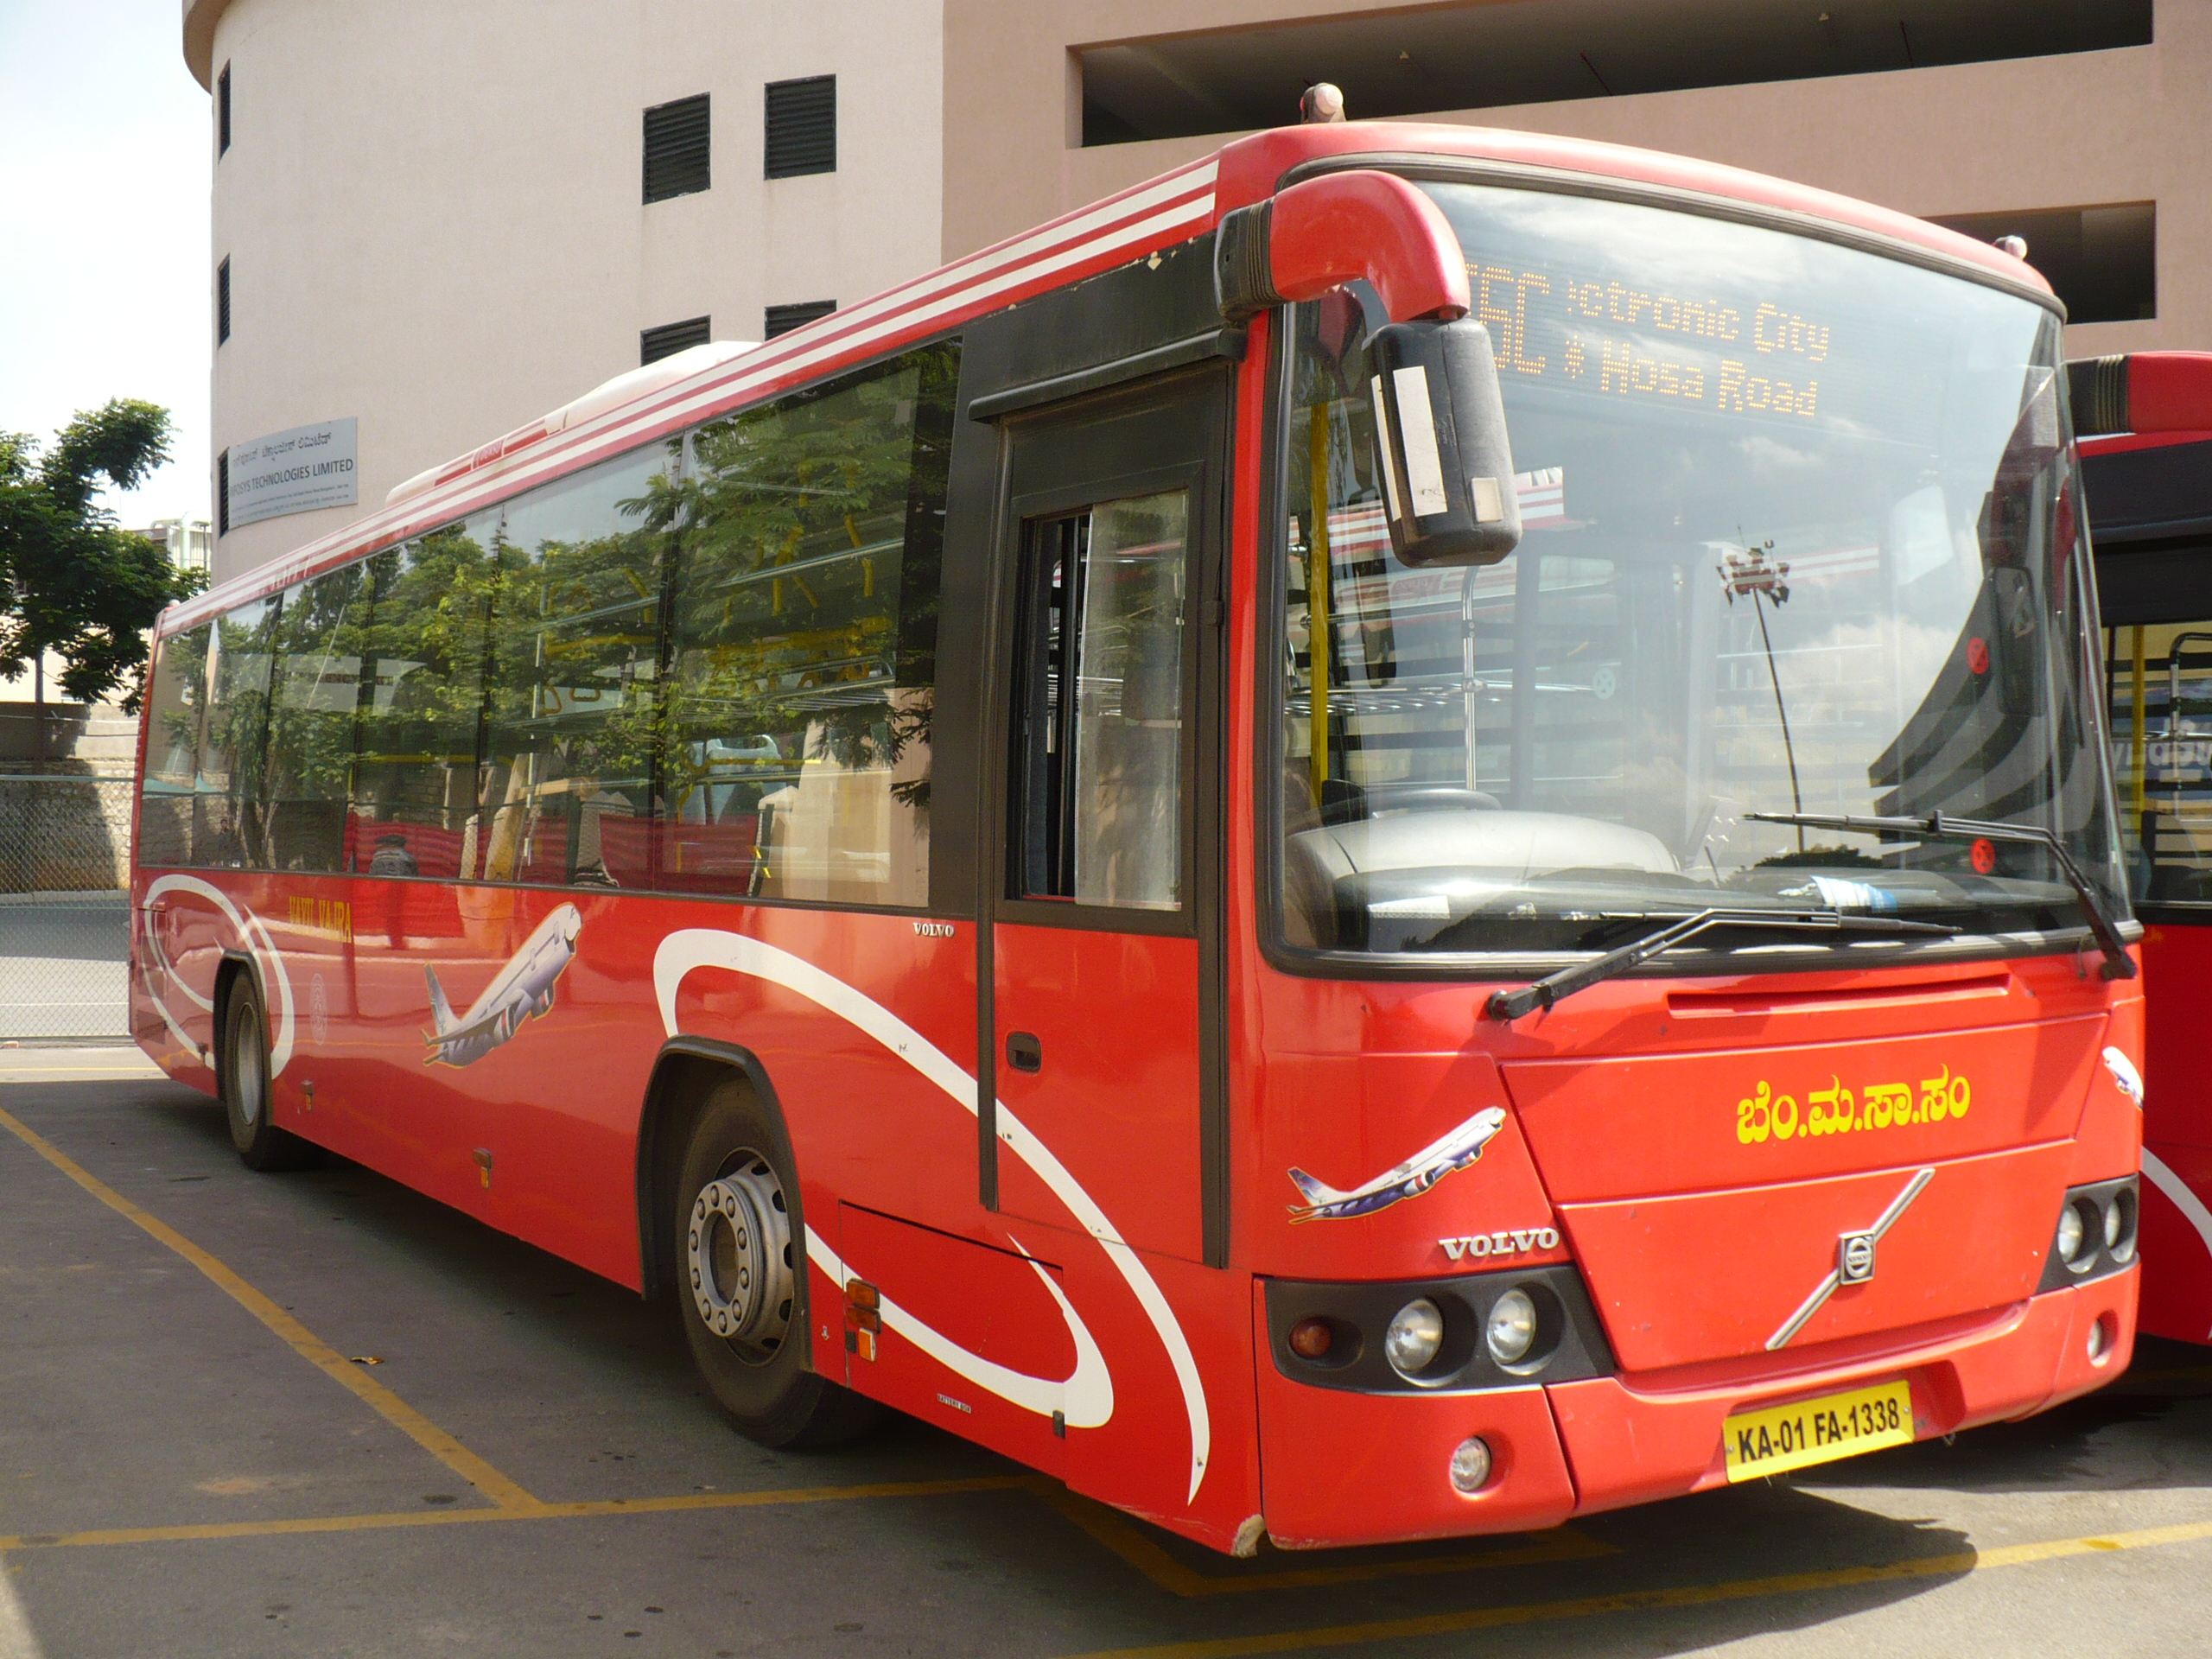
\includegraphics[width=0.45\linewidth,keepaspectratio]{pic/R.jpeg} & 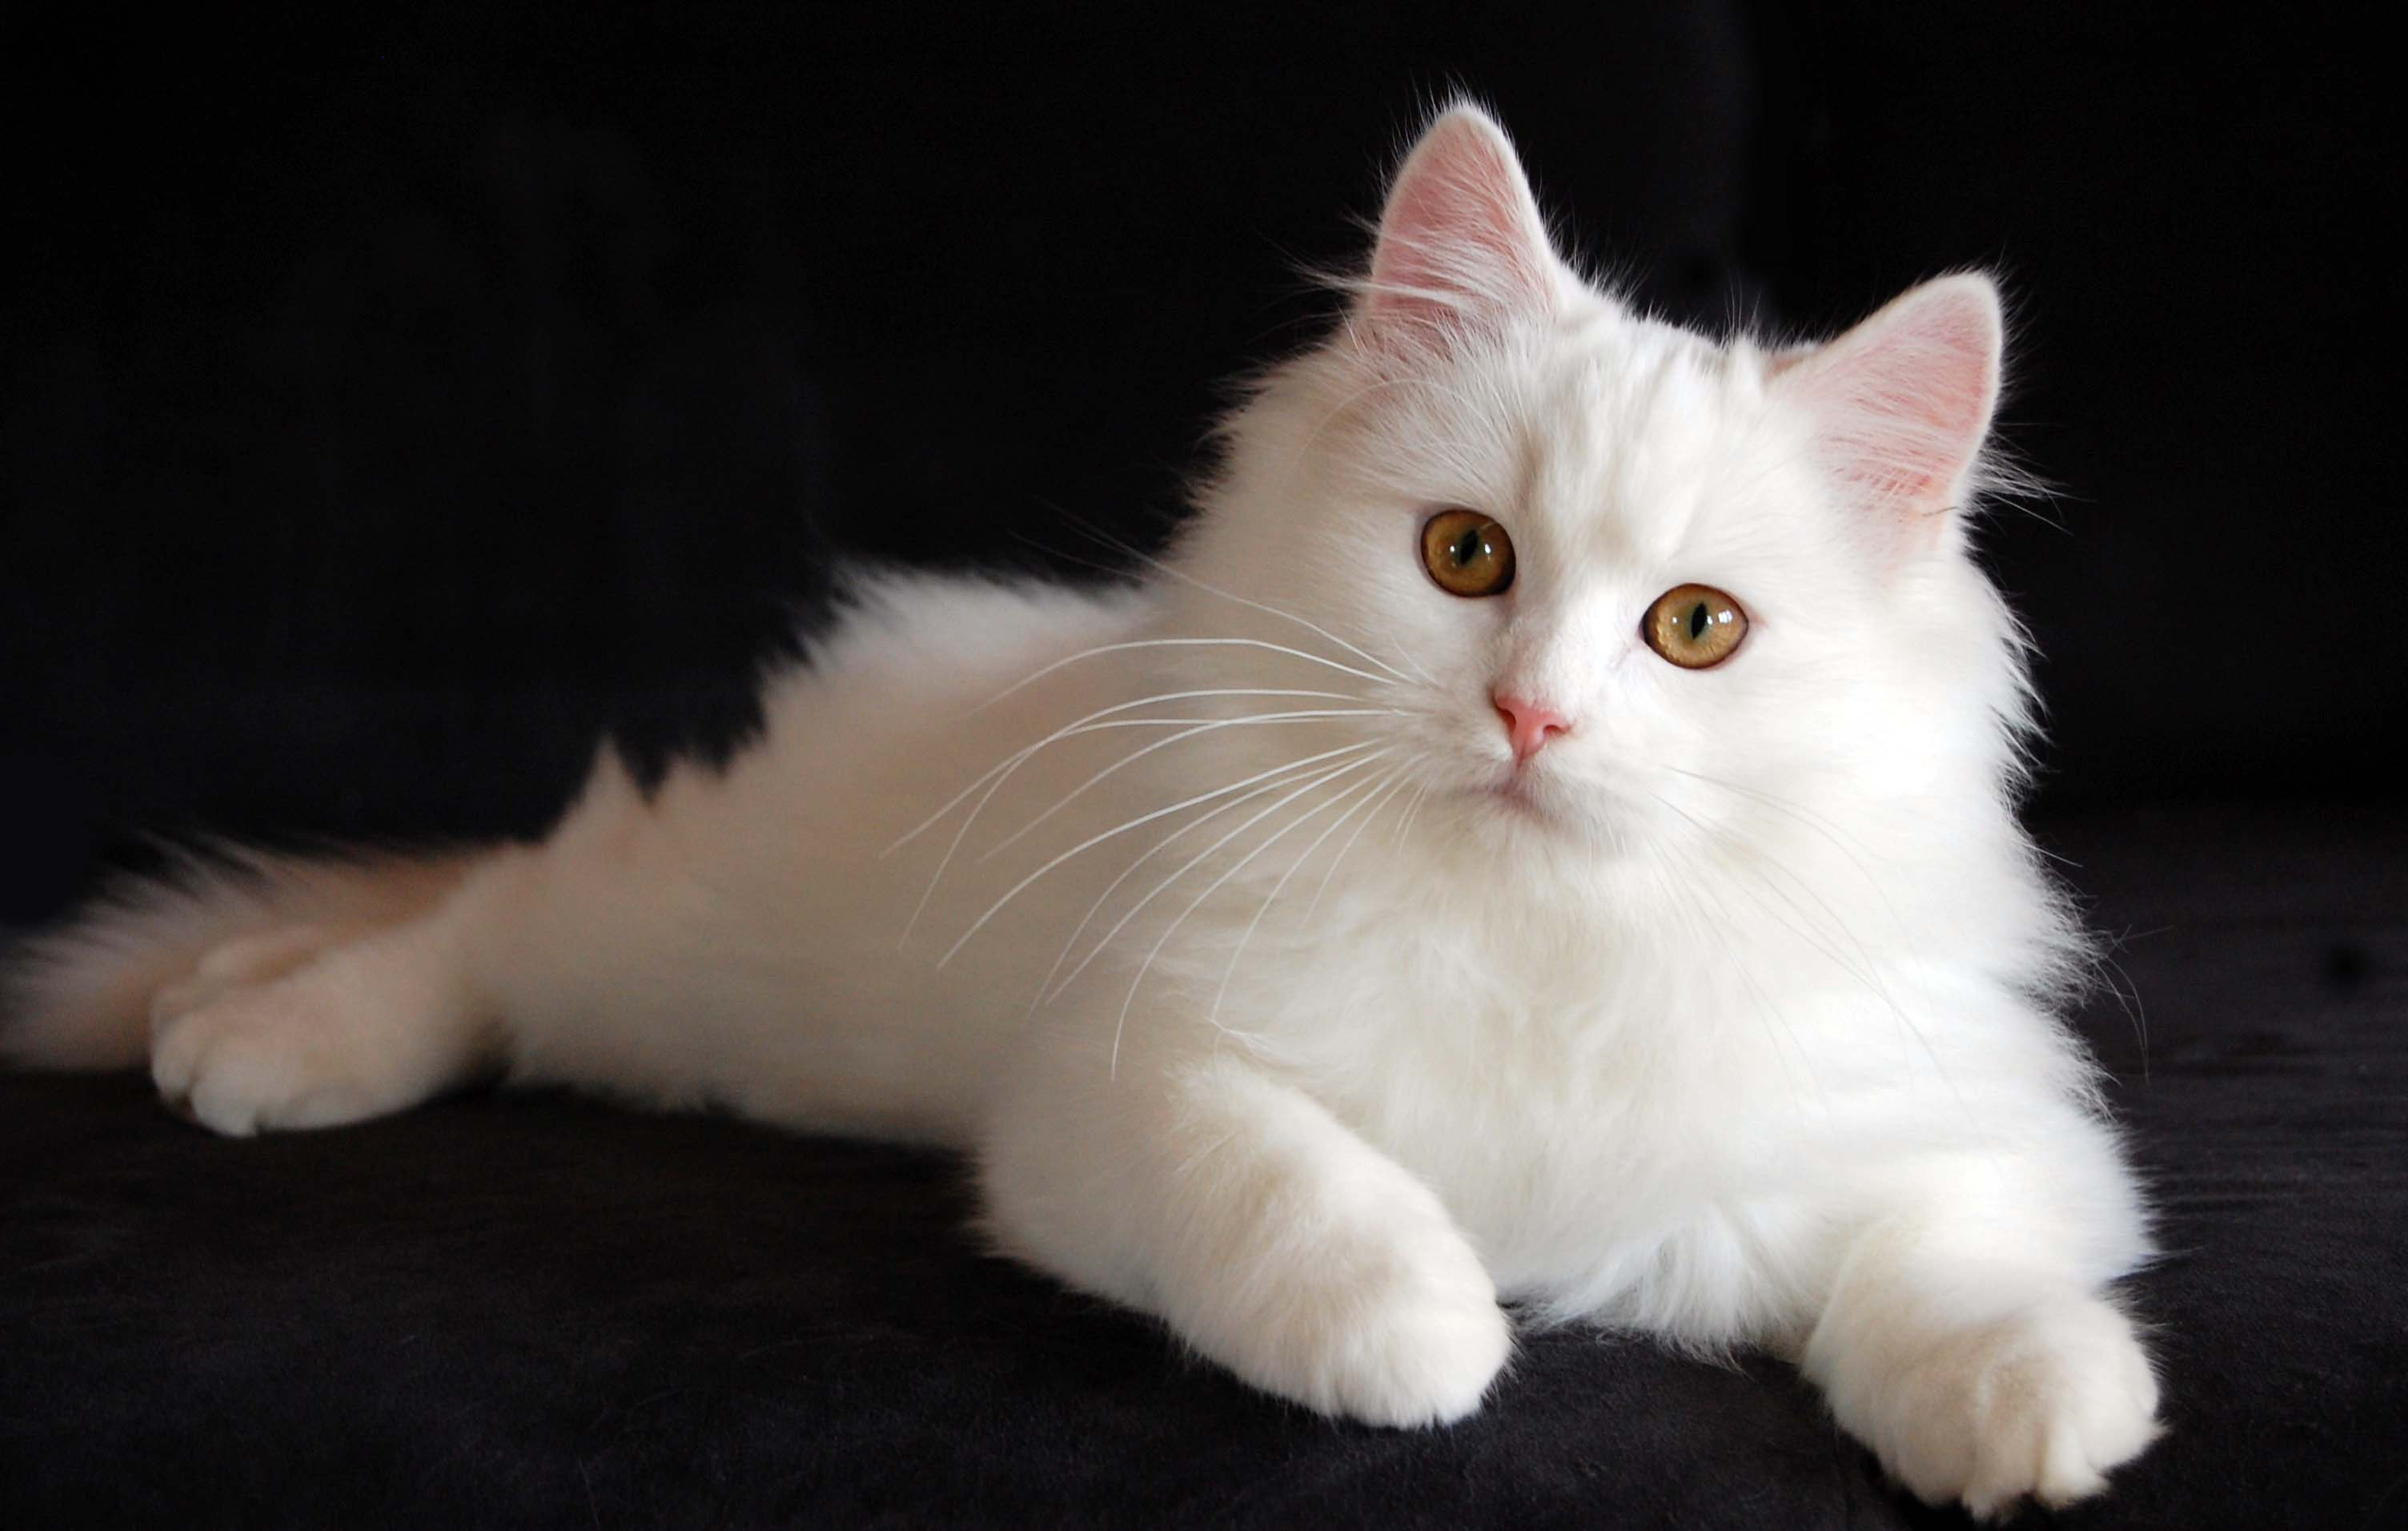
\includegraphics[width=0.45\linewidth,keepaspectratio]{pic/Persian-cat-breed.jpg} \\
    User                                                               & What is related between image 1 and image 2?                                      \\
    \hline
  \end{tabular}
\end{table}

\begin{table}[hbt!]
  \setlength{\extrarowheight}{3pt} % Adjust the value as needed
  \renewcommand{\arraystretch}{1.5} % Adjust the value as needed
  \begin{tabular}{lcccl}
    \hline
    \textbf{Multi Audio Input Example}                                                                                                                     \\[6pt]  % Adjust the value as needed
    \hline
    \hline
    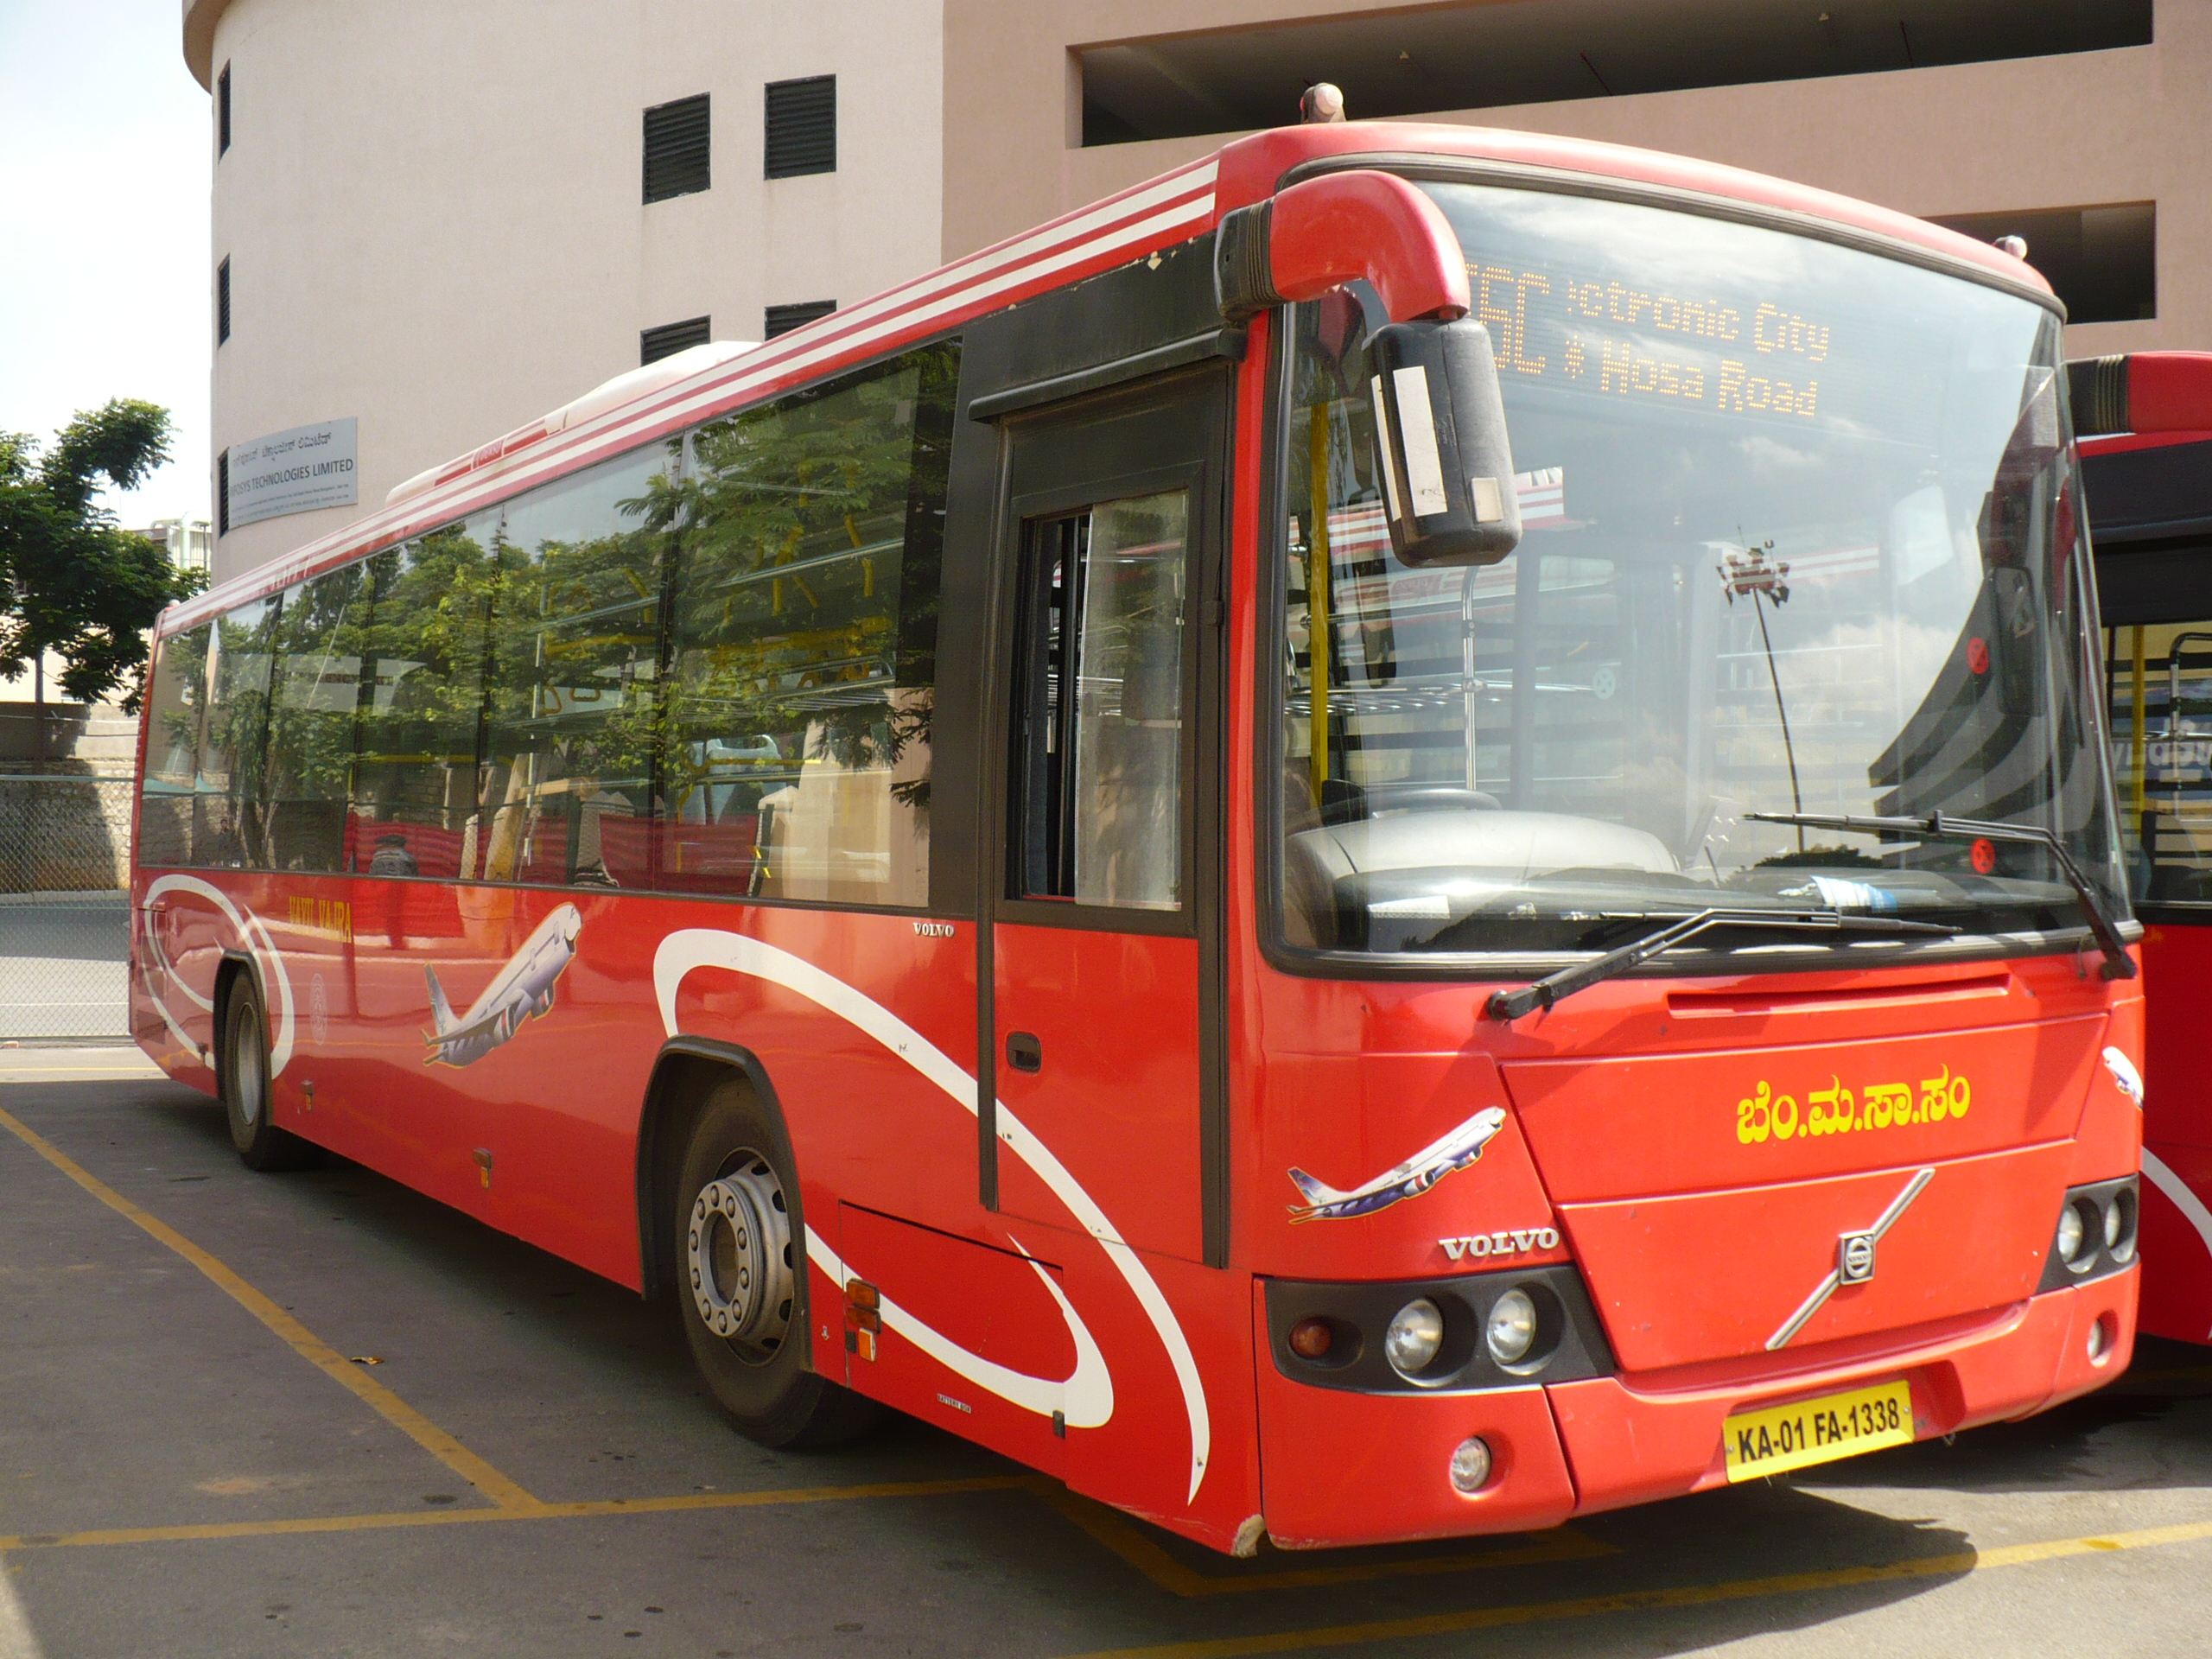
\includegraphics[width=0.45\linewidth,keepaspectratio]{pic/R.jpeg} & 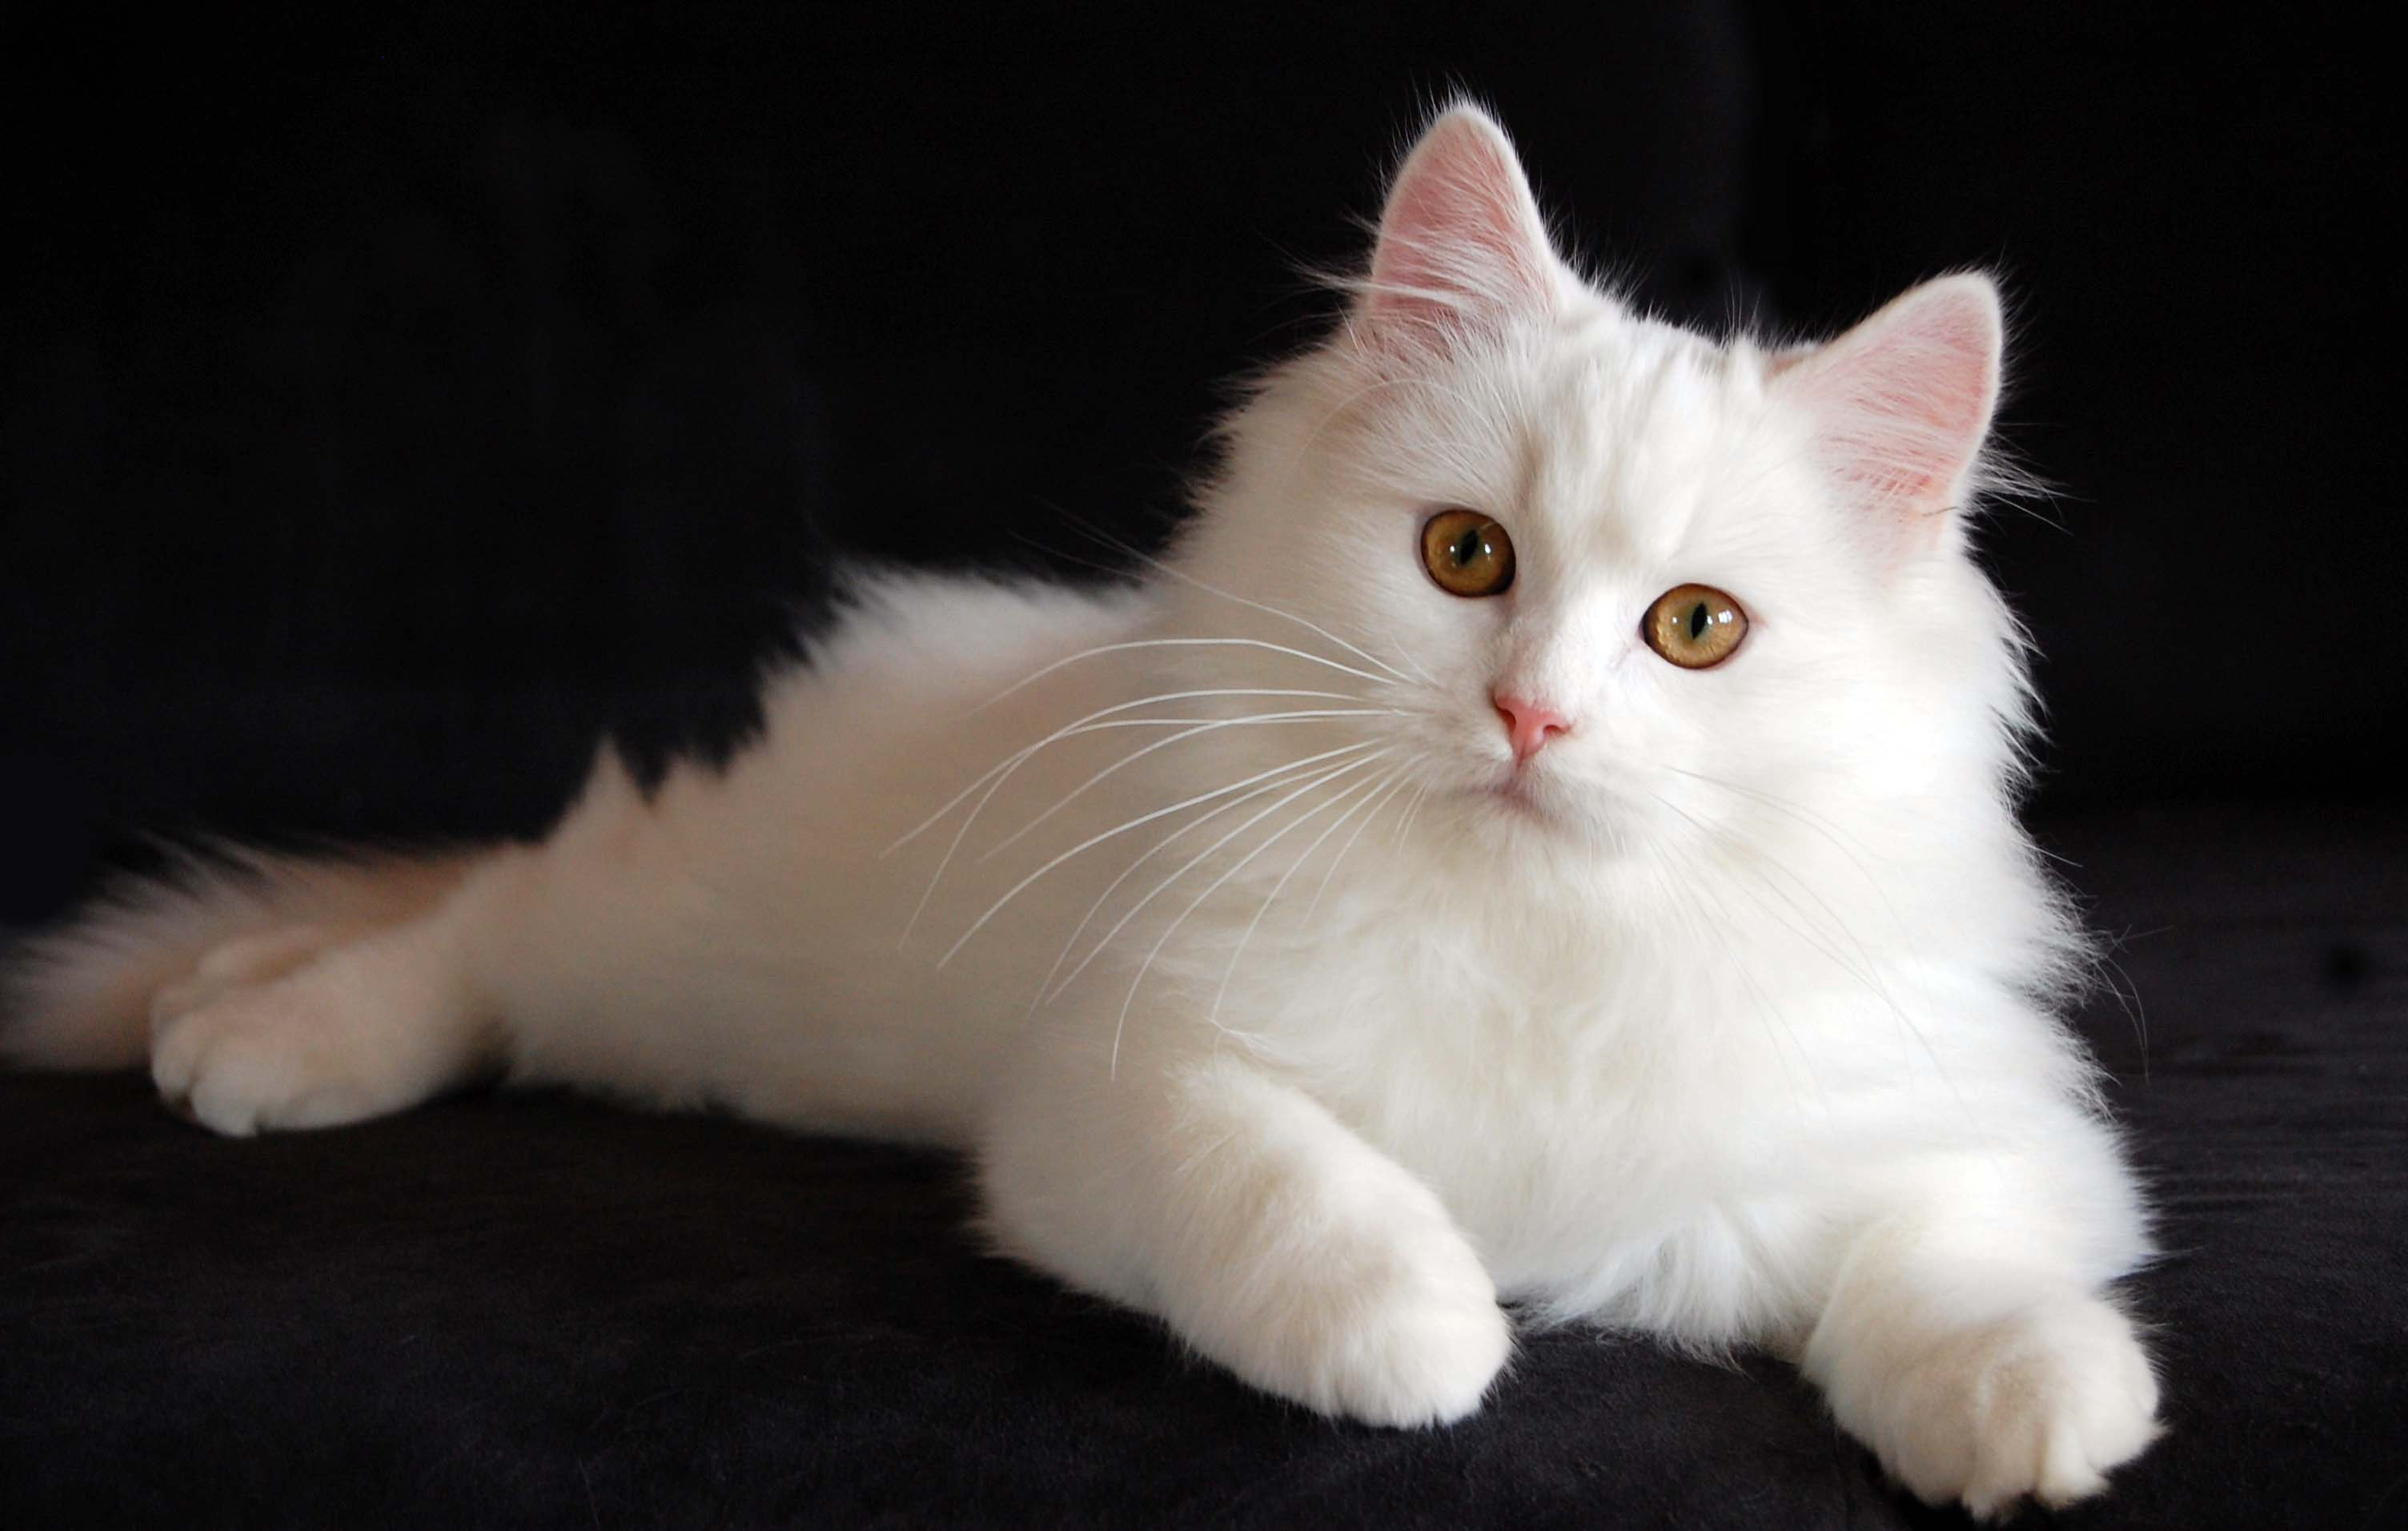
\includegraphics[width=0.45\linewidth,keepaspectratio]{pic/Persian-cat-breed.jpg} \\
    User                                                               & What is related between audio 1 and audio 2?                                      \\
    \hline
  \end{tabular}
\end{table}


\section{Evaluation}

\section{Future Work}

In our future endeavors, we aim to enhance our capabilities by focusing on several key areas. Firstly, we intend to refine our approach to generating synthetic datasets that incorporate multi-images and multi-audio inputs. This will involve expanding the dataset to include more complex relationships between inputs and facilitating comparisons involving more than two inputs. Additionally, we recognize the importance of incorporating a wider range of visual Malaysian context datasets into our model training pipeline. By diversifying our data sources, we can ensure that our model is equipped to handle a broader array of real-world scenarios and contexts, ultimately improving its performance and relevance in practical applications.



\section{Acknowledgement}

Special thanks to Malaysia-AI volunteers especially \href{https://www.linkedin.com/in/wan-adzhar-faiq-adzlan-19a27baa/}{Wan Adzhar Faiq Adzlan}, \href{https://www.linkedin.com/in/ammar-azman/}{Ammar Azman}, \href{https://www.linkedin.com/in/amzar96/}{M. Amzar}, \href{https://www.linkedin.com/in/muhammad-farhan-helmy-0529501a7/}{Muhammad Farhan}, \href{https://www.linkedin.com/in/syafie-nizam/}{Syafie Nizam}, \href{https://www.linkedin.com/in/halimshukor/}{Halim Shukor}, \href{https://www.linkedin.com/in/alif-aiman-1b334b24b/}{Alif Aiman}, \href{https://www.linkedin.com/in/azwan-zuharimi/}{Azwan Zuharimi} and \href{https://www.linkedin.com/in/haziqzikry/}{Haziq Zikry} for contributing dataset to train MMMModal.

We would like to express our gratitude to NVIDIA Inception for generously providing us with the opportunity to train our model on the Azure cloud. Their support has played a crucial role in the success of our research, enabling us to leverage advanced technologies and computational resources.

We extend our thanks to the wider research community for their valuable insights and collaborative discussions, which have greatly influenced our work. This paper reflects the collective efforts and contributions from both NVIDIA Inception and the broader research community.

\section{Conclusion}

In this paper, we introduce MMMModal, a multimodal instruction tuned Model (LLM) specifically designed to handle multiple modalities, including images, audio, and text in a multi-turn dialogue setting. Our novel approach focuses on aligning representations from various modality encoders into a unified space. Unlike existing methods, our approach enables the model to effectively process multi-turn dialogues and incorporate multiple images or audio inputs in its responses. We provide examples demonstrating the multi-modal understanding capabilities of MMMModal.

\bibliography{neurips_2023}{}
\bibliographystyle{unsrt}

\end{document}